\documentclass{article}
\usepackage{polski}
\usepackage[utf8]{inputenc}
\usepackage{indentfirst} 
\usepackage{graphicx} 
\usepackage{pdfpages}
\usepackage{listings}
\newcommand{\HRule}{\rule{\linewidth}{0.5mm}}

\begin{document}

\begin{titlepage}
\begin{center}

% Upper part of the page. The '~' is needed because \\
% only works if a paragraph has started.

\textsc{\LARGE Politechnika Poznańska}\\[1.5cm]

\textsc{\Large Dokumentacja techniczno-rozruchowa}\\[0.5cm]

% Title
\HRule \\[0.4cm]
{ \huge \bfseries PAPAJ \\[0.4cm] }
\textsc{\Large robot typu line-follower}\\[0.5cm]

\HRule \\[1.5cm]

% Author and supervisor
\noindent
\begin{minipage}[t]{0.4\textwidth}
\begin{flushleft} \large
\emph{Autorzy:}\\
Łukasz \textsc{Kosiak} (c)\\
Łukasz \textsc{Królik} \\
Piotr \textsc{Kurzawa} \\
Patryk \textsc{Łapiezo} \\
Sebastian \textsc{Pawlak} \\
Bartosz \textsc{Sławianowski} \\
Kacper \textsc{Stępień} \\
Pedro \textsc{Brêda}
\end{flushleft}
\end{minipage}%
\begin{minipage}[t]{0.4\textwidth}
\begin{flushright} \large
\emph{Prowadzący:} \\
dr. inż. Rafał \textsc{Klaus}
\end{flushright}
\end{minipage}

\vfill

% Bottom of the page
{\large \today}

\end{center}
\end{titlepage}
\tableofcontents
\newpage

\section{Opis}

Papaj jest robotem typu line-follower stworzonym na potrzeby corocznego konkursu RoboDay na Politechnice Poznańskiej, wykonanym przez zdolnych i dumnych studentów z grupy I4.2. 

Nasze urządzenie jest klasycznym przykładem line-followera. Posiada on napęd na tylne koła (każde z nich posiada własny silnik), jest wyposażony w ślizgacze w przedniej części robota oraz 7 czujników linii. Całość jest zasilana popularnymi "paluszkami", co przekłada się na niską cenę.

Papaj został sensacyjnym zwycięzcą RoboDay 2015 w kategorii line-follower zostawiając w tyle bardziej rozbudowane i droższe konstrukcje.

\section{Nazwa}
				
Robocza nazwa Papaja brzmiała "Pommes frites" od napisu, który znajdował się na pudełku, który robił za miejsce jego przechowywania - jednak z powodu niedawnych obchodów 95-rocznicy urodzin Wielkiego Polaka Jana Pawła II, postanowiliśmy nazwać naszego robota na jego cześć. 

Tym samym dołożyliśmy małą cegiełkę w rozpowszechnianie jedynej słusznej prawdy o naszym papieżu. 
						
\section{Budżet}

Jednym z kryteriów, które przyjęliśmy w trakcie projektowania robota była jego cena, która nie powinna przekroczyć 30 zł/os. W związku z tym staraliśmy się maksymalnie ciąć koszty, szukając u siebie i wśród znajomych części, które mogłyby przydać się do zbudowania robota - szczególnie koncentrując się na silniku i zasilaniu. Niestety, zarówno zasilanie, jak i silnik okazały się zbyt mało wydajne i zostaliśmy zmuszeni do zakupu nowych.

Trzeba również zaznaczyć, że nie wszystkie elementy zostały ostatecznie użyte do zbudowania robota (wiele z nich zostało kupione "na zapas") - jednak nie mają one większego wpływu na łączny koszt naszego line-followera.

\begin{table}[c]
\caption{Spis części zakupionych na potrzeby Papaja (ceny w zł)}
\label{table:koszta}
\centering
\begin{tabular}{l|r|r|r}
Element                       & Koszt jedn. & Ilość & Koszt łączny \\
\hline
Transaptor odbiciowy CNY70    & 2,00        & 7     & 14,00        \\
Papier kredowy                & 0,60        & 1     & 0,60         \\
Środek drobnokrystaliczny     & 8,00        & 1     & 8,00         \\
Laminat jednostronny 190x3    & 15,00       & 1     & 15,00        \\
Kondensator ceram. dyskowy    & 0,20        & 12    & 2,40         \\
LED 3mm                       & 0,20        & 3     & 0,60         \\
Sterownik silnika L-293D      & 11,00       & 1     & 11,00        \\
Dławik AL0307                 & 0,20        & 1     & 0,20         \\
Rezystory metaloxide          & 0,20        & 18    & 3,60         \\
20K 0,2W                      & 4,90        & 1     & 4,90         \\
Gniazdo jednorzędowe BLS-09   & 0,45        & 2     & 0,90         \\
Piny do gniazd BLS BL-T       & 0,10        & 24    & 2,40         \\
Gniazda jednorzędowe BLS-02   & 0,10        & 2     & 0,20         \\
Podstawka DIL-28              & 0,50        & 1     & 0,50         \\
Zestaw przewodów              & 7,00        & 1     & 7,00         \\
Płytka stykowa SD12NB         & 14,00       & 1     & 14,00        \\
Listwa 2-rzędowa PLD40        & 1,50        & 1     & 1,50         \\
Bateria 9V                    & 2,60        & 1     & 2,60         \\
BC-639 NPN 100V               & 0,40        & 2     & 0,80         \\
Zacisk do baterii 9V          & 1,60        & 1     & 1,60         \\
Stabilizator napięcia L-7805C & 1,90        & 1     & 1,90         \\
CMOS-4051                     & 1,50        & 1     & 1,50         \\
Rezystory węglowe             & 0,30        & 2     & 0,60         \\
Kondensator 10uF 16V          & 0,50        & 5     & 2,50         \\
LED 5mm                       & 0,40        & 5     & 2,00         \\
Łącznik refl. CNY70           & 5,50        & 1     & 5,50         \\
Kondensator ele. 47uF 16V     & 0,20        & 2     & 0,40         \\
Rezonator kwarcowy 0-16MHz    & 1,80        & 1     & 1,80         \\
Kondesator ele. 22uF 16V      & 0,20        & 2     & 0,40         \\
Dławik radialny 10uH          & 1,30        & 1     & 1,30         \\
ATmega8A-PU DIP28             & 6,99        & 3     & 20,97        
\end{tabular}
\end{table}

Dokładny spis elementów zakupionych na potrzeby Papaja znajduje się w tabeli \ref{table:koszta} na stronie \pageref{table:koszta}.

\section{Schemat ideowy}

\subsection{Jednostka centralna}
Sercem robota jest mikrokontroler ATmega8A-PU. Zdecydowaliśmy się na niego ze względu na cenę, łatwość programowania oraz jego popularność, co miało szczególnie znaczenie podczas problemów z działaniem robota. Doskonała dokumentacja do ATmegi i wiele rozwiązań powszechnie dostępnych w Sieci zdecydowanie ułatwiło nam okiełznanie Papaja i zabezpieczenie go przed niepożądanym działaniem. Poza tym uważamy, że Arduino jest dla słabych i jego wybór mógłby być drogą na skróty, co uwłaszczałoby naszej godności, honorowi i rozumowi człowieka.

Utwierdziliśmy się w przekonaniu, że nasza decyzja była słuszna, gdy okazało się, że naszym wyborem zainspirowało się wiele grup występujących w konkursie RoboDay. Jedna z nich nawet wylądowała na podium, zatem możemy z całą pewnością stwierdzić, że jest to też nasz sukces. Można nawet zaryzykować stwierdzenie, że de facto zajęliśmy dwa miejsca na podium, co wprawia nas w zadumę i zachęca do dalszej pracy.

Jesteśmy przekonani, że nie będzie to nasz ostatni projekt wykorzystujący ten udany układ, a doświadczenie, które uzyskaliśmy w trakcie tworzenia Papaja z pewnością przyda się w przyszłości.



\subsection{Zasilanie}

Zasilanie było zdecydowanie największym wyzwaniem podczas budowy Papaja. Pod uwagę były brane najróżniejsze opcje, łącznie z wykorzystaniem używanych akumulatorków z telefonów marki Nokia (sic!). Zastosowane rozwiązanie, które walnie przyczyniło się do naszego zwycięstwa, przyszło do nas z najmniej spodziewanej strony - sklepu niejakiego  Gembary, który zasugerował nam rozwiązanie "tanio i tanio".

Papaj zasilany jest ośmioma popularnymi paluszkami (baterie AA) połączonymi szeregowo, co zdecydowanie zmniejszyło koszty, zapewniało większą elastyczność i dawało nam całe 12V do wykorzystania. Rozwiązanie to ma jednak dużą wadę - znacząco zwiększa masę robota, co w połączeniu z umiejscowieniem baterii w tylnej części robota powodowało, że Papaj podnosił się i rwał ku radości całego zespołu. 

W celu stabilizowania napięcia dla elektroniki na poziomie 5V zastosowany został stabilizator L-7805C i dał radę.  Silniki natomiast delektowały się pełnym napięciem z baterii wynoszącym 12V.

\subsection{Czujniki odbiciowe}

Papaj w celu wywęszenia linii korzysta z 7 transoptorów CNY70 - ustaliliśmy tę liczbę doświadczalnie w wyniku prób i błędów. Poza tym liczba 7 jest liczbą szczęśliwą i w naszym przypadku sprawdziło się to w stu procentach.

Osobną kwestią był sposób ich połączenia z mikrokontrolerem. Na początku myśleliśmy nad rozwiązaniem programowym, tj. podłączenie sygnału z czujników bezpośrednio do wejść ADC. To rozwiązanie jednak zostało szybko porzucone z paru prozaicznych powodów:
\begin{itemize}
\item ATmega8A-PU ma tylko 6 wejść ADC,
\item programowanie ADC na ATmegach jest niezbyt ciekawe,
\item nie chciało się nam.
\end{itemize}

Stąd też podjeliśmy decyzję o wykorzystaniu rozwiązania sprzętowego, czyli podłączenia transoptorów do zewnętrznych komparatorów (odpowiedzialnych za zamianę sygnału analogowego na cyfrowy), które z kolei są podłączone do wejść cyfrowych ATmegi. 

Ponieważ warunki oświetleniowe w korytarzu BT nie należą do specjalnie dobrych, niezbędne było użycie potencjometru, dzięki któremu poprzez zmianę napięcia odniesienia ustalaliśmy próg decyzji (tj. przejścia między sygnałem 0 i 1). Miało to szczególne znaczenie podczas zawodów, gdyż na trasie białe nie było białe, a czarne też nie było czarne. 

\section{Mechanika}

\subsection{Płytka}
Centralnym elementem, łączącym komponenty robota w całość jest drukowana płytka PCB (Printed Circuit Board). Jej ścieżki zastąpić miały dziesiątki kabli i przewodów łączących elementy. Proces budowy takiej płytki nie jest trudny i skomplikowany, pod warunkiem oczywiście, że człowiek wykona swoją pracę starannie, dokładnie i z pełnym oddaniem.

\subsubsection{Projektowanie}

Płytkę należało zaprojektować w odpowiednio dla tego celu stworzonym programie. Początkowo nasza płytka była tworzona w słynnym EAGLE'u, ostatecznie jednak porzuciliśmy go na rzecz KiCADa, ponieważ jest to narzędzie open-source, a takie oprogramowanie jest szczególnie bliskie naszemu sercu. Niestety, mimo naszej niechęci do zamkniętego oprogramowania nadal byliśmy zmuszeni skorzystać z systemu operacyjnego Windows.  

Projekt ten musiał być wykonany w odbiciu lustrzanym, tak, aby po odbiciu obrazu na płytkę, była ona w prawidłowym położeniu. Aby ułatwić sobie nieco sprawę, umieściliśmy na płytce napis „AKD’15 WI PP” ku chwale Akademii Kreatywnego Działania dr Rafała Klausa.
Prawidłowe odbicie takiego napisu na płytce wskaże, że wszystko poszło jak należy z zaprojektowaniem układu. 

Na wyjściu programu otrzymaliśmy jednostronną płytkę PCB. Niestety sieć połączeń nie zapewniała możliwości poprowadzenia naraz wszystkich połączeń bezkolizyjnie, dlatego też potrzebne było poprowadzenie paru połączeń dodatkowymi kablami. Dzięki temu udało się uniknąć konieczności projektowania znacznie bardziej skomplikowanej konstrukcyjnie płytki dwustronnej. 

\begin{figure}
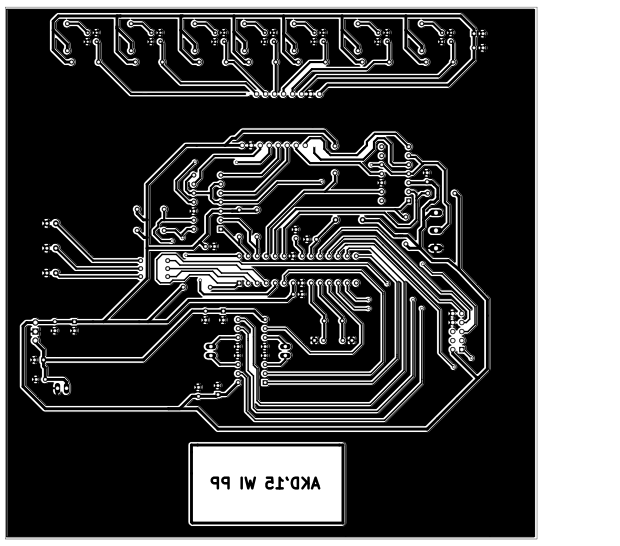
\includegraphics[scale=0.8]{board.png}
\caption{Płytka PCB naszego autorstwa}
\end{figure}
\subsubsection{Drukowanie}

Profesjonaliści biegli w konstruowaniu płytek dysponują sprzętem, który umożliwia konstruowanie płytek o wielu warstwach. Sprzętem takim dysponuje również nasza politechnika, lecz jak się okazało, korzystanie z podobnego sprzętu zostało zakazane. Zostaliśmy zobligowani do metody chałupniczej, tzw. żelazkowej, profesjonalnie nazywaną metodą termotransferową. Drukowanie postępowało w następujących etapach: 

\afterpage{%
\thispagestyle{empty}
\begin{figure}[!htbp]
\centering
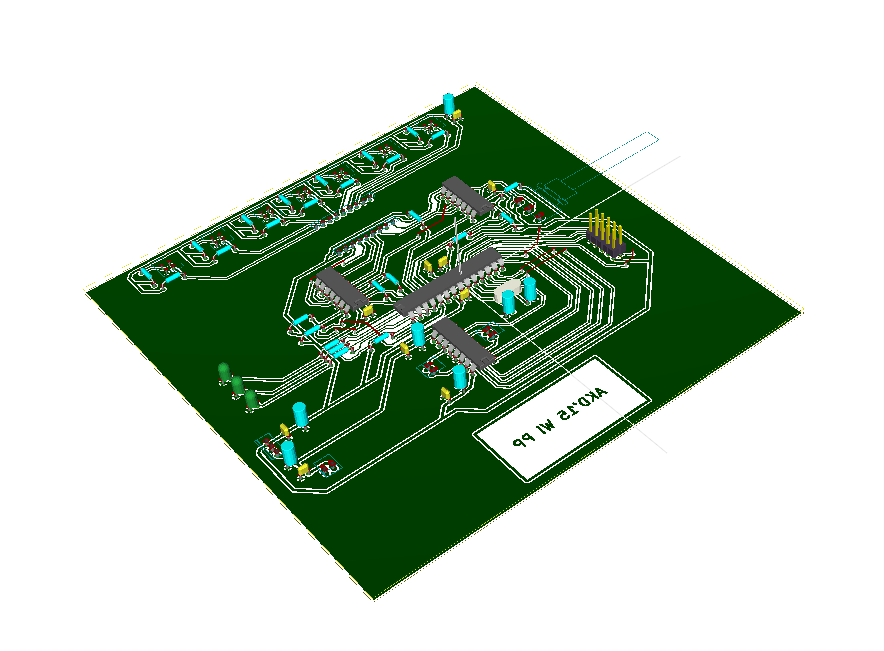
\includegraphics[scale=0.45]{gora.png}
\caption{Płytka PCB - rzut górny}
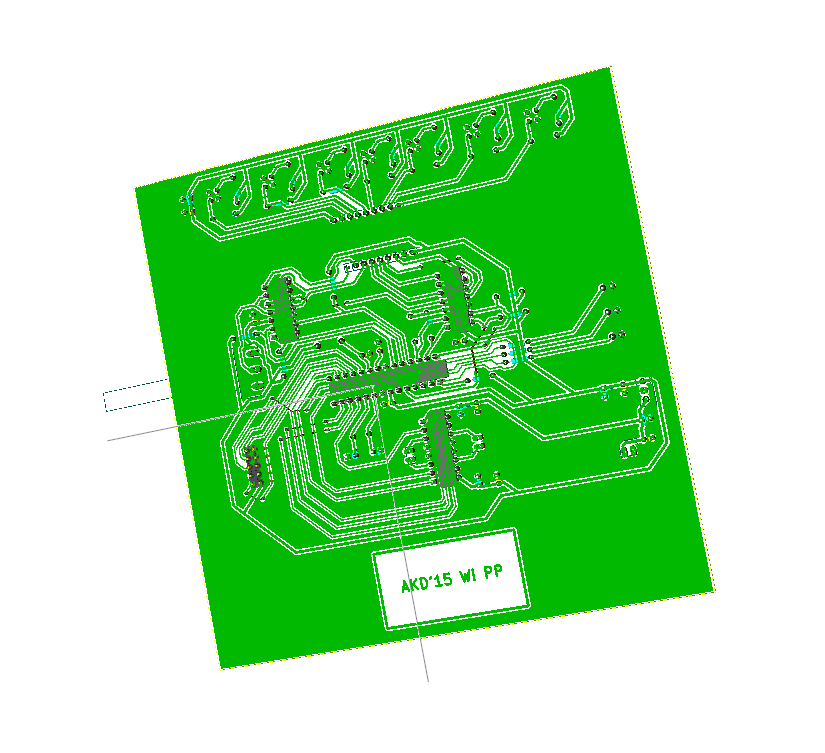
\includegraphics[scale=0.4]{dol.png}
\caption{Płytka PCB - rzut dolny}

\end{figure}
}

\begin{itemize}
\item Wydrukować drukarką laserową, w możliwie jak najlepszej jakości, obraz płytki powstałego w wyniku realizacji punktu 1. Preferowanym typem papieru jest tzw. papier kredowy, którego przewaga nad zwykłym papierem jest taka, że  jego powierzchnia jest bardzo śliska, dzięki czemu słabiej doń przywiera toner.
\item Następnie należy dociąć laminat do rozmiaru wydrukowanego obrazu. Jeśli nie jest on pierwszy raz drukowany, należy go bardzo dokładnie umyć z resztek toneru oraz innych zabrudzeń.
\item Przyłożyć papier kredowy do laminatu i dokładnie nałożyć papier, brzegi zaś kartki nie będące zadrukowane tonerem, użyć do przyklejenia do kartki. Zwrócić uwagę na fałdki papieru, brudy oraz inne podobne defekty.
\item Czwartym krokiem jest ogrzewanie płytki rozgrzanym żelazkiem. Ma ono być możliwie jak najcieplejsze. Dokładnie zgrzać całą powierzchnię kartki, zwracając również uwagę na brzegi kartki, zazwyczaj traktowane po macoszemu. Czas trwania kroku powinien wynosić ok. 15-20 minut. W wyniku okazać się ma, że cały toner został odklejony z papieru i odbił się na miedzianej stronie laminatu.
\item Po intensywnym działaniu termicznym na płytkę, włożyć ją do wody. Można dodać parę kropel detergentu. Płytkę trzymać w wodzie przez około 15 minut - dzięki temu papier zostanie dobrze odmoczony i będzie lepiej odchodzić od tonera. Po odmoczeniu płytki odkleić taśmę klejącą i zdjąć kartkę. Jeśli w wyniku tego nie odejdzie większa część obrazu, można przejść do kolejnego punktu, w przeciwnym razie należy powtórzyć całą procedurę powtórnie. Nasza grupa była zmuszona do trzykrotnego drukowania płytki na nowo. Nie należy zatem zrażać się niepowodzeniami, bo jest to klucz do sukcesu.
\item Następnie należy ostrożnie, z wyczuciem odpowiednim ścierać palcem resztki papieru - TYLKO W MIEJSCACH KTÓRE NIE SĄ POKRYTE CZARNYM TONEREM. Ułatwieniem jest z pewnością to, że białe miejsca nie są do niczego przyklejone, dzięki czemu teoretycznie łatwiej odchodzą. Należy co jakiś czas wkładać ponownie płytkę do wody, z powodu, że woda co jakiś czas znika z powierzchni płytki - głównie przez kontakt z dłońmi oraz w wyniku parowania. Należy uważnie odsłonić ścieżki, tak, że będą one błyszczeć miedzią, z której w rzeczywistości są zbudowane. Jest to najżmudniejsza część metody termotransferowej (nam zajęła około 2 godzin). Metoda ta jest przyczyną bólu rąk, dlatego też ważne jest by działać w zespole oraz wykazać się kreatywnością w konstrukcji narzędzi, np. małego rylca do zdzierania resztek papieru. Pomocą w takim wypadku jest Sz. P. Antonio Vivaldi, którego muzyka pomogła nam przejść ten uciążliwy proces. Serdecznie polecamy jego utwory młodym elektrotechnikom.
\end{itemize}

Przypadki obsługi niewielkich defektów płytki, takich jak zadarcia bądź niepełne odsłonienie ścieżek, zostało omówione w podpunkcie "Uwagi". Zalecamy jednak ostrożność w oczyszczaniu płytki.

\subsubsection{Trawienie}

Należy znaleźć odpowiednie naczynie, w którym umożliwiało zanurzenie w nim płytki w całości. Naczynie winno mieć odpowiednie parametry mechaniczno-chemiczne, takie jak: brak zewnętrznych otworów umożliwiające dyfuzję płynu trawiącego z otoczeniem (np. dziury) czy odporność na rozpuszczenie.

UNDER CONSTRUCTION

\subsubsection{Uwagi}

Często zdarza się, że palec producenta płytki jest zbyt szorstki, tak że zrywa większe połacie tonera, lub jego oko jest na tyle nie uważne, że nie dostrzegł że w którymś miejscu płytki ścieżka jest pokryta papierem. Nie  jest to powód do tego, aby ulec załamaniu nerwowemu oraz innym objawom głębokiej depresji.

W przypadku zdarcia czarnych elementów obrazu płytki, należy zaopatrzyć się w możliwie jak najcieńszy flamaster, o właściwościach zapewniających odporność na wodę. Właściwość ta daje ogromne szanse na to, że również ów tusz oprze się wytrawiaczowi. Należy wówczas dorysować zerwane części obrazu. W przypadku jednak, gdyby metoda ta nie pomogła, należy poprowadzić kabel zwykły między brakującymi ścieżkami. 

Innym defektem jest połączenie się ścieżek, w wyniku niedbałego ściągnięcia papieru z powierzchni płytki. Wówczas może dojść do zwarcia, czyli sytuacji, gdzie przewody nie stykają się w kontrolowany sposób, a raczej gdzieś pośrodku.  Należy problem ten rozwiązać poprzez przecięcie ścieżek nożem. Najlepszy zestaw do badania zwarć składa się z: diody, opornika 240 om, zasilania oraz dwóch przewodów. Należy szeregowo połączyć wszystkie elementy na płytce prototypowej. Przewody powinny być podłączone jednym końcem do obwodu, drugi zaś koniec powinien być wolny. Zetknięcie dwóch przewodów winno zamykać obwód i przyczynić się do zaświecenia diody - należy tak zbudowany zestaw obsłużyć. Jeden przewód powinien być przyłożony do masy, czyli do zewnętrznego obszaru płytki, nie mającego nic prócz miedzi, zaś drugim powinno się sprawdzać ścieżki układu, pilnując by nie zapaliła się dioda. W przypadku jej zapalenia łatwo wykazać, że doszło do zwarcia, i należy tą sytuację skorygować.

\subsection{Układ jezdny}
Napęd robota składa się z dwóch silniczków. Ich działanie opiera się na metodzie różnicowej, stosowanej chociażby w czołgach. Każde koło jest oddzielnie napędzane i skręt wynika z tego, że jedno koło kręci się szybciej od drugiego. W tym celu został wykorzystany układ L293, który miał na celu sterowanie pracą silników. Regulacja prędkości obrotowej kół odbywa się poprzez PWM (regulację współczynników wypełnienia).

Ruch kółek czerpie się z działania silniczków elektrycznych, których szybkość jest zależna od ilości napięcia, jakie zostanie dostarczone na styki. Konieczną procedurą było zatem sprawienie, że ruch silniczka miałby wpływ na ruch kółka. Należało skonstruować jakiś mechanizm przeniesienia jednego ruchu na drugi. 

„Należało” - słowo to padło nieprzypadkowo, ponieważ zaniechaliśmy konstrukcji własnej roboty. Byłby to mechanizm niedoskonały, który znacznie spowolniłby robota z powodu niedoskonałości technicznych układu przełożenia. Z tego też powodu postanowiliśmy zainwestować więcej pieniędzy w silniczki, które miało gotową zębatkę dopasowaną do dołączonego kółka. Układ ten bardzo dobrze się sprawdził, nie „gubił” kroków i dzięki temu robot nasz mógł poruszać się tempem bardzo szybkim.

Najprostsza jednak wersja napędu opiera się na przekładni pasowej zbudowanej z popularnej gumki recepturki. Daje ona rezultaty, jest do tego opcją budżetową i ekonomiczną, jednakże ma mały współczynnik tarcia statycznego i nie może osiągnąć zachwycającej prędkości. Rozwiązanie dylematu prędkość vs. koszty zostawiamy Czytelnikowi, którego bardzo serdecznie pozdrawiamy. Osoby posiadające zabawki mogą się również postarać o sprawdzenie, czy z ich komponentów nie dałoby się stworzyć napędu. Przydatne byłby wszelkiego rodzaju zębatki. Ważna jest kreatywność, otwarty umysł i wiara we własne możliwości. 




\subsection{Model 3D}

\section{Kod źródłowy}

Algorytm opiera się na zasadzie działania regulatora PID. W każdej iteracji (około 3000 na sekundę) program sprawdza, który najbardziej skrajny czujnik wykrywa linię. Każdemu czujnikowi przypisane są odpowiednie wagi - po prawej stronie robota są dodatnie, a po lewej ujemne.
Następnie wyliczane są wartości członów: 
\begin{itemize}
\item proporcjonalnego (bezpośrednio wskazującego na kierunek, w którym znajduje się linia),
\item różniczkującego (odpowiedzialnego za nagłą zmianę kierunku jazdy),
\item całkującego (odpowiedzialnego za stopniowe zmniejszanie promienia skrętu w wypadku pokonywania długiego zakrętu).
\end{itemize}

Ich suma podstawiana jest do zmiennej \emph{steeringValue},  której wartość następnie zmniejsza/zwiększa się tak, aby mieściła się w przedziale (-1000; 1000).
Jeśli jest ujemna (czyli robot powinien skręcać w lewo), ustawiana jest maksymalna prędkość prawego koła, a prędkość lewego jest pomniejszana o wartość bezwzględną \emph{steeringValue}. 
Jeśli jest dodatnia (czyli robot powinien skręcać w prawo), ustawiana jest maksymalna prędkość lewego koła, a prędkość prawego jest pomniejszana o wartość bezwzględną \emph{steeringValue}.

Przy bardzo ostrych skrętach robot wyjeżdża poza linię (stan zerowy wszystkich czujników). W takim wypadku, aby przyspieszyć jego powrót (który normalnie zostałby również wykonany, dzięki członowi całkującemu), tymczasowo ignorowana jest wartość \emph{steeringValue} i uruchomiona zostaje procedura przywracania robota na trasę, poprzez wykonanie gwałtownego skrętu w stronę ostatniego czujnika, pod którym wcześniej wykryta była linia, tj. w wypadku ostrego skrętu w prawo prędkość lewego koła jest ustawiana na maksymalną, natomiast prawe koło jest przez krótki okres wycofywane, co jeszcze bardziej zmniejsza promień skrętu. Po ponownym wykryciu linii program powraca do normalnej pracy.

Prędkość kół ustawiana jest za pomocą metod \emph{setLeftMotorPwm} oraz \emph{setRightMotorPwm}, przyjmujących wartości z zakresu od 0 do 1000 i przekształcających je liniowo do przedziału opisywanego przez stałe \emph{lmin}, \emph{lmax} lub \emph{rmin} oraz \emph{rmax}, które definiują minimalne oraz maksymalne wypełnienie sygnału PWM na wyjściu do odpowiedniego silnika. Przykładowo przy ustawieniu:

\begin{lstlisting}
const int lmin = 0;
const int rmin = 0;
const int rmax = 380;
const int lmax = 400;
\end{lstlisting}
wywołanie funkcji:
\begin{lstlisting}
setLeftMotorPwm(900);
\end{lstlisting}
spowodowałoby ustawienie wysokiej prędkości dla lewego silnika (wypełnienie PWM = 360).


\section{Podziękowania}

Na wstępie chcielibyśmy podziękować naszemu prowadzącemu, dr. inż. Rafałowi Klausowi,  za nieocenione wsparcie i wkład w budowę naszego robota. Jesteśmy dumni ze współpracy z dr. Klausem i mamy cichą nadzieję, że również on jest z naszej pracy dumny.

Dziękujemy także Maciejowi Uniejewskiemu i Mateuszowi Sarbinowskiemu, którzy  wytykając nam brak ambicji i odrzucając naszą propozycję współpracy, zachęcili nas do tytanicznej pracy zakończonej pełnym sukcesem. Mamy nadzieję, że taka sytuacja w przyszłości się nie powtórzy - choć obiecujemy, że tego Wam nigdy nie zapomnimy. Z litości nie będziemy wspominać, jakie pozycje w konkursie zajęły grupy, do których dwie powyższe jednostki należały.

Nie możemy zapomnieć również o Janie Pawle II, który dawał nam inspirację i chęci do tworzenia robota, pomimo wszelkich przeciwności losu.

Na koniec pragniemy serdecznie podziękować grupie tworzącej robota "Mały, ale wariat" z Aleksandrą Kobus na czele. Doprawdy rzadko zdarza się sytuacja, aby grupa, która sama tworzyła trasę finalną i miała przywilej testowania swojego robota na swojej trasie parę dni przed zawodami, zawody te przegrała. Szczerze gratulujemy.

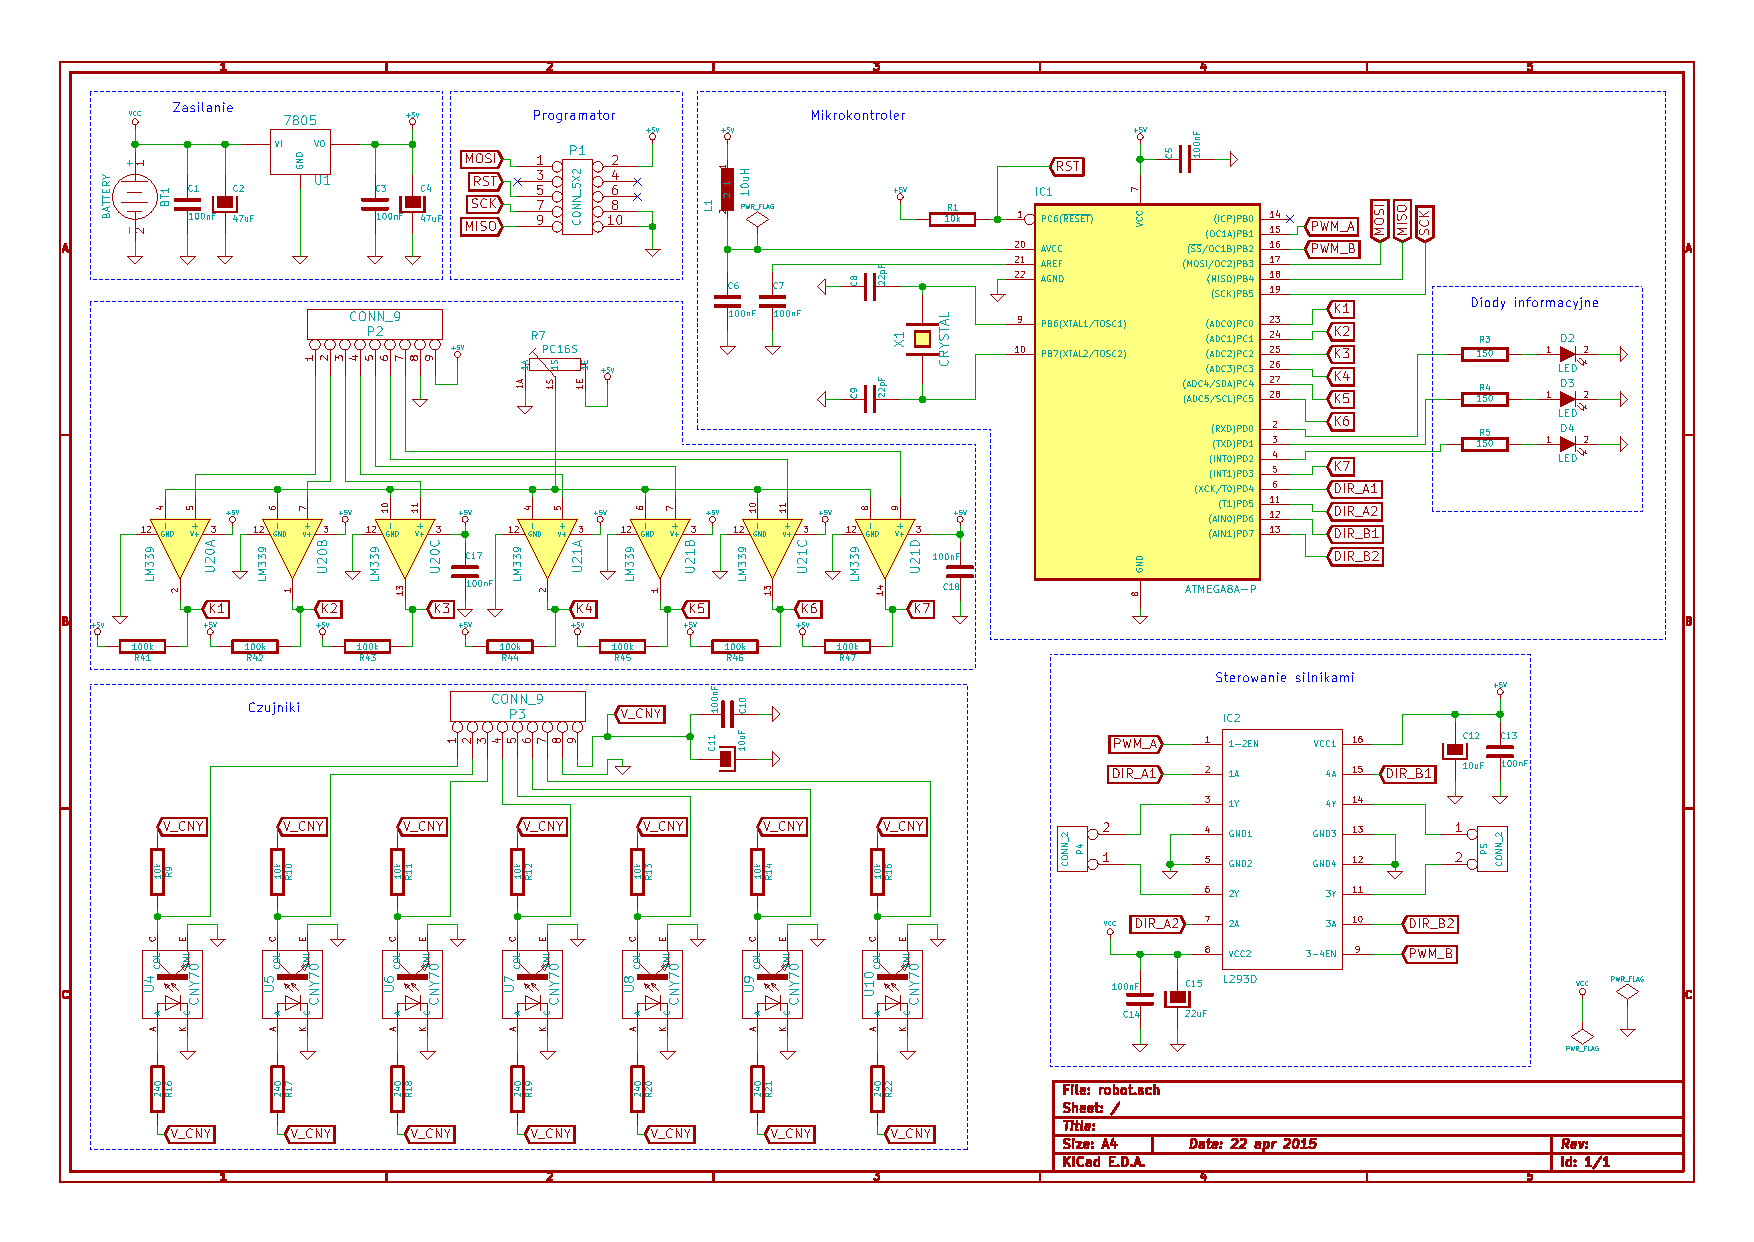
\includepdf[pages={1},angle=-90]{kicad.pdf}

\end{document}

